
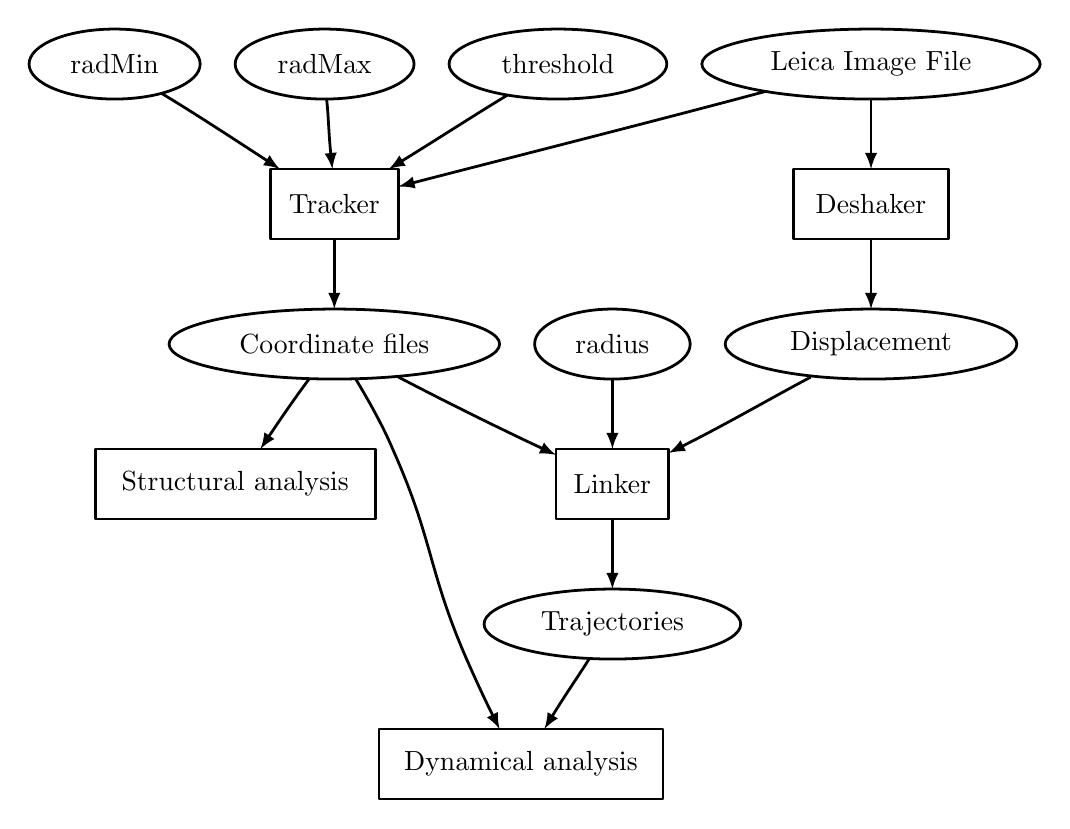
\begin{tikzpicture}[>=latex,line join=bevel,scale=0.7]
  \pgfsetlinewidth{1bp}
%%
\pgfsetcolor{black}
  % Edge: dat_files -> Linker
  \draw [->] (190bp,217bp) .. controls (211bp,206bp) and (239bp,192bp)  .. (271bp,177bp);
  % Edge: threshold -> Tracker
  \draw [->] (246bp,362bp) .. controls (231bp,353bp) and (211bp,340bp)  .. (185bp,324bp);
  % Edge: lif -> Tracker
  \draw [->] (379bp,364bp) .. controls (327bp,350bp) and (248bp,330bp)  .. (190bp,315bp);
  % Edge: dat_files -> Structure
  \draw [->] (144bp,216bp) .. controls (138bp,208bp) and (131bp,198bp)  .. (119bp,180bp);
  % Edge: radMax -> Tracker
  \draw [->] (153bp,360bp) .. controls (154bp,352bp) and (154bp,343bp)  .. (156bp,324bp);
  % Edge: dat_files -> Dynamics
  \draw [->] (168bp,216bp) .. controls (174bp,206bp) and (182bp,192bp)  .. (187bp,180bp) .. controls (208bp,133bp) and (205bp,118bp)  .. (225bp,72bp) .. controls (229bp,63bp) and (233bp,54bp)  .. (242bp,36bp);
  % Edge: lif -> Deshaker
  \draw [->] (433bp,360bp) .. controls (433bp,352bp) and (433bp,343bp)  .. (433bp,324bp);
  % Edge: Tracker -> dat_files
  \draw [->] (157bp,288bp) .. controls (157bp,280bp) and (157bp,271bp)  .. (157bp,252bp);
  % Edge: displ_file -> Linker
  \draw [->] (402bp,217bp) .. controls (383bp,207bp) and (359bp,193bp)  .. (329bp,178bp);
  % Edge: radMin -> Tracker
  \draw [->] (68bp,363bp) .. controls (83bp,354bp) and (103bp,341bp)  .. (129bp,324bp);
  % Edge: radius -> Linker
  \draw [->] (300bp,216bp) .. controls (300bp,208bp) and (300bp,199bp)  .. (300bp,180bp);
  % Edge: Deshaker -> displ_file
  \draw [->] (433bp,288bp) .. controls (433bp,280bp) and (433bp,271bp)  .. (433bp,252bp);
  % Edge: Linker -> traj_file
  \draw [->] (300bp,144bp) .. controls (300bp,136bp) and (300bp,127bp)  .. (300bp,108bp);
  % Edge: traj_file -> Dynamics
  \draw [->] (288bp,72bp) .. controls (283bp,64bp) and (276bp,54bp)  .. (265bp,36bp);
  % Node: radMin
\begin{scope}
  \pgfsetstrokecolor{black}
  \draw (44bp,378bp) ellipse (44bp and 18bp);
  \draw (44bp,378bp) node {radMin};
\end{scope}
  % Node: lif
\begin{scope}
  \pgfsetstrokecolor{black}
  \draw (433bp,378bp) ellipse (87bp and 18bp);
  \draw (433bp,378bp) node {Leica Image File};
\end{scope}
  % Node: displ_file
\begin{scope}
  \pgfsetstrokecolor{black}
  \draw (433bp,234bp) ellipse (75bp and 18bp);
  \draw (433bp,234bp) node {Displacement};
\end{scope}
  % Node: Linker
\begin{scope}
  \pgfsetstrokecolor{black}
  \draw (329bp,180bp) -- (271bp,180bp) -- (271bp,144bp) -- (329bp,144bp) -- cycle;
  \draw (300bp,162bp) node {Linker};
\end{scope}
  % Node: dat_files
\begin{scope}
  \pgfsetstrokecolor{black}
  \draw (157bp,234bp) ellipse (85bp and 18bp);
  \draw (157bp,234bp) node {Coordinate files};
\end{scope}
  % Node: traj_file
\begin{scope}
  \pgfsetstrokecolor{black}
  \draw (300bp,90bp) ellipse (66bp and 18bp);
  \draw (300bp,90bp) node {Trajectories};
\end{scope}
  % Node: Tracker
\begin{scope}
  \pgfsetstrokecolor{black}
  \draw (190bp,324bp) -- (124bp,324bp) -- (124bp,288bp) -- (190bp,288bp) -- cycle;
  \draw (157bp,306bp) node {Tracker};
\end{scope}
  % Node: radius
\begin{scope}
  \pgfsetstrokecolor{black}
  \draw (300bp,234bp) ellipse (40bp and 18bp);
  \draw (300bp,234bp) node {radius};
\end{scope}
  % Node: threshold
\begin{scope}
  \pgfsetstrokecolor{black}
  \draw (272bp,378bp) ellipse (56bp and 18bp);
  \draw (272bp,378bp) node {threshold};
\end{scope}
  % Node: Dynamics
\begin{scope}
  \pgfsetstrokecolor{black}
  \draw (326bp,36bp) -- (180bp,36bp) -- (180bp,0bp) -- (326bp,0bp) -- cycle;
  \draw (253bp,18bp) node {Dynamical analysis};
\end{scope}
  % Node: Deshaker
\begin{scope}
  \pgfsetstrokecolor{black}
  \draw (473bp,324bp) -- (393bp,324bp) -- (393bp,288bp) -- (473bp,288bp) -- cycle;
  \draw (433bp,306bp) node {Deshaker};
\end{scope}
  % Node: Structure
\begin{scope}
  \pgfsetstrokecolor{black}
  \draw (178bp,180bp) -- (34bp,180bp) -- (34bp,144bp) -- (178bp,144bp) -- cycle;
  \draw (106bp,162bp) node {Structural analysis};
\end{scope}
  % Node: radMax
\begin{scope}
  \pgfsetstrokecolor{black}
  \draw (152bp,378bp) ellipse (46bp and 18bp);
  \draw (152bp,378bp) node {radMax};
\end{scope}
%
\end{tikzpicture}

